\section{Data handling and processing system}

\subsection{The protoDUNE Data Characteristics}

The design of the Liquid Argon TPC has a few fundamental properties which affect the data characteristics in the experiment:
\begin{itemize}
\item High spatial granularity of readout (e.g. the electrode pattern), and the resulting high channel count
\item High digitization frequency (which is essential to ensure a precise position measurement along the drift direction)
\item Relatively slow drift velocity of electrons in Liquid Argon, which  leads to a substantial readout window (of the order of milliseconds) required to collect
all of the ionization in the Liquid Argon volume due the event of interest. 
\end{itemize}

\noindent
Combination of these factors leads to a considerable amount of data per event and depending on
the chosen conditions (i.e. trigger rate and total required statistics) may result in considerable requirements
regarding the bandwidth and storage. These issues will be addressed in the sections below.

%There are a few data reduction (compression) techniques that may be applicable to \pd raw data in order to reduce its size. Some of the algorithms
%are inherently lossy, such as the so-called \textit{Zero Suppression} algorithm which rejects parts of the digitized waveforms in LArTPC channels according
%to certain logic (e.g. when the signal is consistently below a predefined threshold for a period of time). There are also lossless compression
%techniques such as Huffman algorithm and others. At the time of writing it is assumed that only the lossless algorithms will be applied
%during the compression
%of the \pd raw data, while zero suppression is considered a separate option that may be implemented when taking a portion of the data.

%It is foreseen that the total amount of data to be produced by the \pd detectors will be of the order of a few
%petabytes (including commissioning runs with cosmic rays). Instantaneous and average data rates in the data transmission chain are expected to be
%substantial (see \ref{sec:np02_online_processing} and \ref{sec:np04_data_rate}).
%For these reasons, capturing data streams generated by the protoDUNE DAQ systems, buffering of the data, performing fast QA analysis,
%and transporting the data to sites external to CERN for processing (e.g. FNAL, BNL, etc.) requires significant resources and adequate planning.



%%%%%%%%%%%%%%% Tom's stuff

The constraints on the data handling and processing system are
determined most directly by the desired data rate and, to a lesser
extent, the total data volume.  The data rate depends on the number of
triggers needed in order to meet the test and measurement goals, and
the operating schedule.  Available funding and personnel also place
constraints on the size and functionality of the online data handling
and processing system.

In order to meet the physics requirements with an amount of
contingency to allow for commissioning and schedule delays, the DAQ
and online processing system is designed to handle an instantaneous
trigger rate of 100~Hz.  All six APA modules are to be read out on
each trigger.  The data are assumed to be compressed in the RCE's,
with a lossless compression ratio of 5.  Data are assumed to be
collected based on prompt trigger signals generated by the beamline
instrumentation in order to purify samples of desired particles.

The readout of the photon detector channels and the beam
instrumentation is assumed to be a relatively minor addition to the
total data rate and are not anticipated to drive the design of the
data handling and processing system, although adequate resources must
be provisioned in order to acquire and store the data from these
systems.  The network speed of all computers in the data acquisition
chain is anticipated to be 10 GBits/sec.  Computers running near-line
processing of subsets of the data, which are generally CPU-bound, may
be connected with 1~GBit/sec links.  The software framework for
interfacing with the electronics, building events, writing data files,
and providing an interface to online monitoring of data as it is
acquired is {\it artdaq}~\cite{artdaq}.

Assuming that each RCE reads out 128 channels of the TPC, 120 RCE's
will need to be active.  Twelve computers running BoardReader
processes will read out ten RCE's each.  These computers should be
provisioned with at least 8 cores and 16 GBytes of RAM each, along
with a 10 GBit/sec network connection.  The BoardReader processes will
transmit data to a set of computers running EventBuilder processes.
Sixteen EventBuilder computers, each with 8 cores and 16 GBytes of RAM
and a 10 GBit/sec NIC will provide the CPU and networking needed to
build events, perform basic online monitoring, and send the data to
disk storage.  The EventBuilders assemble data fragments sent by the
BoardReaders into self-consistent events consisting of readout data
from each contributing RCE, SSP, and beam instrumentation information
for the same time period.  They will also perform basic data integrity
checks, ensuring that all data that are expected for an event have
arrived and have not been corrupted, before writing records out.

The disk storage layer will consist of 350 TBytes of high-speed
network-attached disks.  As of this writing, the filesystem and
interface software layer is not yet defined, but may be one of the
following -- an instance of EOS~\cite{eos}, XRootD~\cite{xrootd}, or
simply disks locally attached to the EventBuilder computers.  A
alternative to this design that allows for more flexibility but at a
cost of network latency and CPU, is to add a layer of Aggregator CPU
processes between the EventBuilders and the disk writing.  These
processes may be needed if the events are to be sorted, analyzed,
reformatted, or otherwise handled before writing out.  In order to
maximize throughput and minimize cost, the number of steps in the data
handling system is to be minimized.

After the data are written to disk by {\it artdaq}, the data handling
system creates metadata files, runs near-line monitoring jobs, and
transfers the data from EHN1 to the CERN Computing Centre, as
described in DUNE DocDB~1212~\cite{docdb1212}.

\begin{figure}[tbh]
\centering
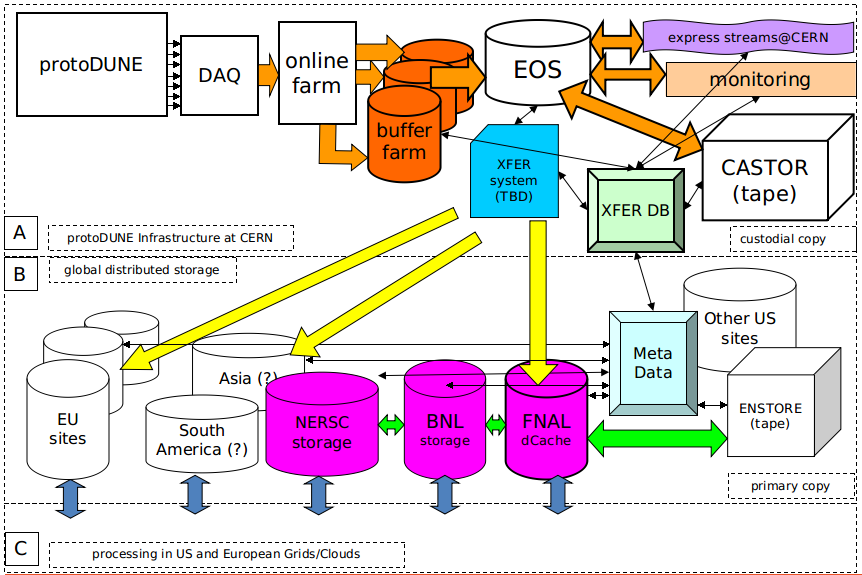
\includegraphics[width=\linewidth]{figures/protoDUNE_raw_data_concept.png}
\caption{\label{fig:raw_concept}Conceptual diagram of the flow of raw data in protoDUNE}
\end{figure}

